%-----------------------------------------------------------------------------%
\chapter{\babEmpat}
%-----------------------------------------------------------------------------%
Bab ini menjelaskan secara detail proses implementasi dari pengolahan data, proses \textit{pattern extraction} dan \textit{matching}, pembobotan dan \textit{ranking} baik \textit{pattern} maupun \textit{pair}.

%-----------------------------------------------------------------------------%
\section{Pembentukan Korpus Kalimat Wikipedia}
%-----------------------------------------------------------------------------%
\begin{figure}
    \centering
    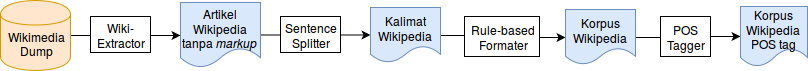
\includegraphics[width=\linewidth]{pics/Pic02-PreProcessingWikipedia}
    \caption{Pre-processing Data Wikipedia}
    \label{fig:preproses-wiki}
\end{figure}
Data hasi Wikipedia Dump diformat secara otomatis menggunakan \textit{tools} WikiExtractor. WikiExtractor adalah program berbasis Python yang dibuat oleh Giuseppe Attardi dan Antonio Fuschetto. Menggunakan \textit{tools} ini, didapatkan data yang sudah tidak mengikuti format MediaWiki Markup, Language. Program ini dapat diunduh dari Github dan dijalankan menggunakan perintah berikut. 

\begin{lstlisting}[caption={Penggunaan Wiki Extractor}, language=bash]
$ WikiExtractor.py xml-dump-file -o output-file
\end{lstlisting}

\noindent Jika tidak memberi spesifikasi opsi apapun, artikel yang dihasilkan membersihkan seluruh markup, language dan hanya menyimpan isi artikel tanpa disertakan informasi seperti kategori, riwayat, dan versi artikel.

%-----------------------------------------------------------------------------%
\subsection{Sentence Splitting}
%-----------------------------------------------------------------------------%
Korpus yang dihasilkan menghasilkan baris-baris yang merepresentasikan suatu paragraf dalam artikel Wikipedia. Pada penelitian kali ini, ingin dilihat relasi \textit{hypernym-hyponym} antar dua kata pada kalimat yang sama. Untuk itu, perlu dilakukan proses \textit{sentence splitting} yang dapat mengidentifikasi suatu kalimat dalam paragraf. Hasil dari proses tersebut adalah dokumen yang terdiri dari baris-baris yang merepresentasikan satu kalimat. 

Proses ini dilakukan dengan menggunakan \textit{script} yang telah dibuat sebelumnya oleh Ken Nabila Setya dari Fasilkom UI, Indonesia. Ditambah pula satu \textit{script} yang dapat secara otomatis melakukan \textit{splitting} untuk seluruh dokumen. Berikut adalah contoh sebuah paragraf dalam artikel Wikipedia yang telah dibersihkan menggunakan WikiExtractor.
\begin{center}
\begin{tabular}{ | m{32em} | } 
\hline
Charles Anthony Johnson (3 Juni 1829 - 17 Mei 1917), kemudian dikenal sebagai Charles Brooke memerintah Sarawak sebagai Raja Putih kedua dari 3 Agustus 1868 hingga meninggal dunia. Dia menggantikan pamannya, James Brooke sebagai raja. \\
\hline 
\end{tabular}
\end{center}

\noindent Setelah melalui proses \textit{sentence splitter}, berikut adalah hasilnya.
\begin{center}
\begin{tabular}{ | m{32em} | } 
\hline
Charles Anthony Johnson (3 Juni 1829 - 17 Mei 1917), kemudian dikenal sebagai Charles Brooke memerintah Sarawak sebagai Raja Putih kedua dari 3 Agustus 1868 hingga meninggal dunia. \\
\hline 
 Dia menggantikan pamannya, James Brooke sebagai raja. \\
\hline
\end{tabular}
\end{center}

%-----------------------------------------------------------------------------%
\subsection{Rule Based Formatter}
%-----------------------------------------------------------------------------%
Dari korpus yang berisi kalimat Wikipedia, diberikan beberapa aturan tambahan untuk membuat korpus sesuai format yang diinginkan. Penambahan aturan juga untuk mengurangi ambiguitas dan bentuk usaha generalisasi \textit{pattern}. Berikut adalah beberapa aturan tambahan untuk \textit{pre-processing} korpus Wikipedia.
\begin{enumerate}
  \item Menghilangkan frasa yang berada di dalam tanda kurung. \\
  Frasa yang terletak di dalam tanda kurung dapat dianggap sebagai penjelas kata atau frasa sebelumnya. Proses ini merupakan salah satu upaya generalisasi \textit{pattern}.
  \item Memisahkan simbol-simbol yang berhimpit pada awal dan akhir kata. \\
  Beberapa token yang dipisahkan oleh spasi dalam kalimat merupakan kata yang berhimpit dengan tanda baca. Untuk mempermudah proses selanjutnya yaitu \textit{sentence tagging}, dilakukan \textit{pre-processing} tambahan yaitu memisahkan simbol-simbol \textit{non-alphanumerical}.
  \item Memberi penanda awal kalimat dengan '<start>'' dan akhir kalimat dengan '<end>'. \\
  Pemberian simbol awal dan akhir kalimat memperjelas isi kalimat dan juga menunjang proses \textit{pattern extraction} dan \textit{pattern matching}.
\end{enumerate}

\noindent Dari contoh kalimat di atas, setelah melalui proses \textit{formatting} yang didefinisikan menghasilkan kalimat berikut.
\begin{center}
\begin{tabular}{ | m{32em} | } 
\hline
<start> Charles Anthony Johnson , kemudian dikenal sebagai Charles Brooke memerintah Sarawak sebagai Raja Putih kedua dari 3 Agustus 1868 hingga meninggal dunia . <end> \\
\hline 
<start> Dia menggantikan pamannya , James Brooke sebagai raja . <end> \\
\hline
\end{tabular}
\end{center}


%-----------------------------------------------------------------------------%
\section{POS Tagging Kalimat Wikipedia}
%-----------------------------------------------------------------------------%
Proses \textit{part-of-speech tagging} dilakukan pada korpus Wikipedia yang telah berbentuk kalimat dengan format yang didefinisikan. Pada penelitian ini, kelas kata yang menjadi pengamatan adalah \textit{noun} (NN) dan \textit{proper noun} (NNP), sehingga proses \textit{pos tagging} digunakan untuk identifikasi kata-kata tersebut. Proses \textit{pos tagging} menggunakan \textit{tools} Stanford POS Tagger, dengan model yang digunakan merupakan hasil penelitian sebelumnya menggunakan Bahasa Indonesia.  Setelah selesai melalui proses \textit{tagging}, dilakukan penyesuaian agar format korpus lebih rapi dan terstruktur. 

Berikut adalah contoh kalimat yang sudah melalui tahap \textit{pos tagging}. Korpus ini digunakan untuk proses \textit{pattern matching}.
\begin{center}
\begin{tabular}{ | m{32em} | } 
\hline
<start>\_X Charles\_NNP Anthony\_NNP Johnson\_NNP ,\_Z kemudian\_CC dikenal\_VB sebagai\_IN Charles\_NNP Brooke\_NNP memerintah\_VB Sarawak\_NNP sebagai\_IN Raja\_NNP Putih\_NNP kedua\_CD dari\_IN 3\_CD Agustus\_NNP 1868\_CD hingga\_IN meninggal\_VB dunia\_NN .\_Z <end>\_X \\ 
\hline
\end{tabular}
\end{center}


%-----------------------------------------------------------------------------%
\section{Seed Builder}
%-----------------------------------------------------------------------------%
\begin{figure}
    \centering
    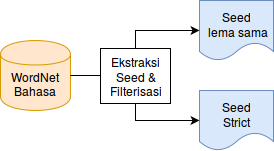
\includegraphics[scale=0.6]{pics/Pic02-SeedBuilder}
    \caption{Proses Pembentukan \textit{Seed}}
    \label{fig:seed-builder}
\end{figure}
Proses pengumpulan \textit{seed} dibantu dengan \textit{resource} yang dimiliki WordNet Bahasa menggunakan \textit{tools} nltk. Proses pengumpulan diawali dengan mengambil seluruh lema Bahasa Indonesia yang dimiliki oleh korpus nltk. Setelah itu, ambil seluruh \textit{synset} yang mengandung lemma tersebut. Dari setiap \textit{synset}, ambil relasi \textit{hypernym}-nya. Dari setiap \textit{synset hypernym}, ambil lema Bahasa Indonesianya. Dilakukan pula filterisasi \textit{synset} ataupun lema untuk mengurangi ambiguitas. Untuk setiap \textit{synset} maupun lema yang diambil pada setiap tahapan, hanya boleh berasal dari kelas kata kerja (\textit{noun}). Setelah didapatkan, bentuk ke dalam pasangan \textit{tuple} 1-1 $(kata\_hyponym,kata\_hypernym)$.
%--- kode seed builder ----- %
\begin{lstlisting}[caption={Algoritme pembentukan \textit{seed}}, language=bash]
buildSeed:
  ambil seluruh lemma bahasa indonesia noun
  untuk setiap lema:
    ambil seluruh synset dari lema tersebut
    untuk setiap synset:
      ambil seluruh synset hypernym
      untuk setiap synset hypernym 
        ambil seluruh lemma hypernym
        untuk setiap lemma hypernym:
          filterisasi
          bentuk pasangan lemma-lemma hypernym
\end{lstlisting}
%--------------------------- %

%-----------------------------------------------------------------------------%
\subsection{Filterisasi Seed}
%-----------------------------------------------------------------------------%
Filterisasi dilakukan dengan tujuan mengurangi ambiguitas, namun tetap berusaha mendapatkan \textit{seed} sebanyak mungkin. Filterasisasi juga dilakukan untuk mendapatkan \textit{seed} awal yang diyakini benar dan berkualitas. Salah satu bagian terpenting proses ini adalah memasangkan hanya lema yang merupakan \textit{noun} ke lema yang juga adalah \textit{noun}. Jika kemungkinan lema tersebut tergolong ke dalam kelas kata bukan \textit{noun}, lema tidak diikutsertakan sebagai \textit{seed} awal.

Tantangan dalam proses ini adalah banyak ditemukan kasus dimana satu lema dikandung oleh lebih dari satu \textit{synset} atau satu \textit{synset} memiliki lebih dari satu \textit{synset hypernym}. Ambiguitas dalam kasus tersebut dapat mengurangi kualitas \textit{seed} yang dihasilkan. Mengatahui hal tersebut, dibuatlah dua pendekatan berbeda untuk proses filterisasi \textit{seed}.

Pendekatan pertama adalah tetap mengambil lemma yang sama pada \textit{synset hypernym} yang berbeda. Hal ini dilatarbelakangi adanya lema yang berasal dari \textit{synset} berbeda namun memiliki lema \textit{hypernym} yang sama. Pada contoh (i), satu lema yang sama dimiliki oleh dua \textit{synset} yang berbeda namun kedua \textit{synset} tersebut memiliki \textit{synset hypernym} yang sama. Lema untuk kedua \textit{synset hypernym} adalah sama sehingga tetap diikutsertakan sebagai \textit{seed}. Pada contoh (ii), satu lema berasal dari dua \textit{synset} yang berbeda dan dua \textit{synset hypernym} berbeda, namun ada lema yang sama yaitu 'laluan'.

Pendekatan lainnya adalah dengan metode filterisasi yang \textit{strict}. Jika satu lema memiliki lebih dari satu \textit{synset hypernym}, maka lema tersebut dianggap ambigu dan langsung tidak diikutsertakan ke dalam \textit{seed} awal. Berdasarkan tabel contoh lema, \textit{synset}, dan \textit{hypernym}-nya, hanya contoh (i) yang diterima sebagai \textit{seed} karena \textit{synset hypernym} untuk lema tersebut sama. Sementara (ii) ditolak karena \textit{synset hypernym} berbeda.

\begin{center}
\begin{tabular}{ |c|m{30em}| } 
\hline
\multirow{2}{*}{i.} & ('paruh', Synset('beak.n.02')) => (['bibir', 'kuala', 'muara'], [Synset('mouth.n.02')])
('paruh', Synset('beak.n.01')) => (['bibir', 'kuala', 'muara'], [Synset('mouth.n.02')]) \\ 
& ('paruh', Synset('beak.n.01')) => (['bibir', 'kuala', 'muara'], [Synset('mouth.n.02')]) \\ 
\hline
\multirow{2}{*}{ii.} & ('pintu\_masuk', Synset('entrance.n.01')) => (['akses', 'capaian', 'laluan'], [Synset('access.n.03')]) \\ 
& ('pintu\_masuk', Synset('orifice.n.01')) => (['koridor', 'laluan', 'lorong'], [Synset('passage.n.07')]) \\ 
\hline
\end{tabular}
\end{center}


%-----------------------------------------------------------------------------%
\section{Sentence Tagging}
%-----------------------------------------------------------------------------%
Setelah memperoleh pasangan kata relasi Bahasa Indonesia, perlu dilakukan \textit{tagging} pasangan kata tersebut ke kalimat-kalimat dalam korpus Wikipedia. Data yang digunakan untuk proses ini adalah korpus Wikipedia tanpa \textit{pos tag}. Beberapa tahapan dilakukan pada proses \textit{tagging sentence} dengan pasangan kata relasi adalah sebagai berikut.
\begin{enumerate}
  \item Dibaca seluruh pasangan kata relasi \textit{hyponym-hypernym}.
  \item Untuk setiap kalimat pada korpus Wikipedia, di cek apakah kalimat tersebut mengandung pasangan kata relasi.
  \item Pengecekan dilakukan secara berulang untuk seluruh pasangan kata relasi karena terdapat kemungkinan satu kalimat mengandung lebih dari satu pasang kata relasi.
  \item Kata-kata yang merupakan bagian dari pasangan kata relasi kemudian di-\textit{tag} sesuai relasinya dan disimpan ke dalam korpus berisi kalimat dengan \textit{tag} \textit{hyponym} dan \textit{hypernym}.
\end{enumerate}
Pada penelitian ini, satu kalimat yang telah di-\textit{tag} hanya mengandung tepat satu pasangan kata relasi. Untuk kasus khusus dimana suatu pasangan kata relasi terdiri dari satu kata yang merupakan sub kata pasangannya, maka pasangan kata tersebut tidak diikutsertakan untuk menghindari ambiguitas. Contoh pasangan kata yang tidak diikutsertakan adalah $(ikan\,\,gurame;ikan)$, kata 'ikan' terkandung dalam kedua kata relasi.
%--- kode sentence tagging ----- %
\begin{lstlisting}[caption={Algoritme \textit{sentence tagging}}, language=bash]
tagAll:
  seeds = load_all_seeds()
  foreach sentence in sentences:
    tagSentence(sentence, seeds)

tagSentece(sentence, seeds):
  foreach seed in seeds:
    if (sentence.contains(seed.hypernym) && sentence.contains(seed.hyponym)):
      put_tag_hyponym()
      put_tag_hypernym()
      save_sentence()
\end{lstlisting}
%------------------------------ %

Berikut adalah contoh kalimat yang terbentuk dari proses \textit{sentence tagging}. Diberikan pasangan kata relasi \textit{hyponym-hypernym} $(fermion;partikel)$ dan $(boson;partikel)$ serta kalimat  '<start> seluruh partikel dasar adalah boson atau fermion . <end>'. Hasil proses \textit{sentence tagging} adalah sebagai berikut.
\begin{center}
  \begin{tabular}{ | m{32em} | } 
  \hline
    <start> seluruh <hypernym>partikel<hypernym> dasar adalah boson atau <hyponym>fermion<hyponym> . <end> \\ \hline
    <start> seluruh <hypernym>partikel<hypernym> dasar adalah <hyponym>boson<hyponym> atau fermion . <end> \\ \hline
  \end{tabular}
\end{center}

\begin{figure}
    \centering
    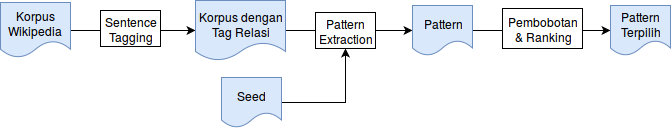
\includegraphics[width=\linewidth]{pics/Pic03-PatternExtraction}
    \caption{Proses Pembentukan \textit{Pattern}}
    \label{fig:pattern-extraction}
\end{figure}

%-----------------------------------------------------------------------------%
\section{Pattern Extraction}
%-----------------------------------------------------------------------------%
Setelah mendapatkan kalimat-kalimat yang telah di-\textit{tag} dengan kata relasi, ingin dicari \textit{pattern} yang dapat digunakan untuk menambah jumlah relasi kata. Pembuatan \textit{pattern} menggunakan algoritma dasar \textit{standard trie} dengan beberapa modifikasi. Proses ini diimplementasi secara mandiri menggunakan program Java dengan mengikuti algoritma pembuatan \textit{Trie} sederhana.

Suatu \textit{\textit{node}} merepresentasikan kata dalam kalimat dan dari satu kalimat terbentuk sebuah cabang dalam \textit{tree}. \textit{Node} menyimpan beberapa informasi seperti nama \textit{\textit{node}}, \textit{parent}, \textit{childs}, dan informasi identitas tambahan seperti apakah \textit{\textit{node}} tersebut merupakan relasi (\textit{hypernym} atau \textit{hyponym}) dan apakah \textit{\textit{node}} tersebut merupakan \textit{leaf}. Untuk kata yang merupakan kata relasi, \textit{\textit{node}} menyimpan informasi jenis relasi beserta \textit{list} dari kata yang merupakan bagian dari relasi tersebut. 

\noindent Sebagai contoh dua kalimat sebagai berikut.
\begin{center}
  \begin{tabular}{ | m{32em} | } 
  \hline
  <start> <hyponym>singa<hyponym> adalah <hypernym>kucing<hypernym> yang berukuran besar <end> \\ \hline
  \hline
  <start> <hyponym>serigala<hyponym> adalah <hypernym>anjing<hypernym> yang tinggal di hutan <end>\\ \hline
  \end{tabular}
\end{center}

\noindent Akan menghasilkan \textit{Pattern} Tree sebagai berikut. Angka setelah kata adalah bobot suatu \textit{node}.

\begin{lstlisting}[caption={Contoh \textit{pattern tree} yang terbentuk}, language=bash]
`-^ (1)
 `-<hyponym> (2)
   `-adalah (2)
     `-<hypernym> (2)
       `-yang (2)
        |-berukuran (1)
        | `-besar (1)
        `-tinggal (1)
          `-di (1)
            `-hutan (1)
\end{lstlisting}

%-----------------------------------------------------------------------------%
\subsection{Informasi dalam Pattern}
%-----------------------------------------------------------------------------%
Beberapa informasi yang disimpan dalam suatu \textit{pattern} adalah \textit{sequence} kata yang merepresentasikan \textit{pattern} tersebut, jumlah kemunculan dalam korpus, \textit{seed} unik yang membentuk \textit{pattern}, dan kalimat unik yang membentuk \textit{pattern}. Informasi-informasi tersebut digunakan untuk pembentukan vektor \textit{pattern}, pemberian bobot \textit{pattern} dan melakukan \textit{sorting} untuk mendapatkan \textit{pattern} terbaik.

%-----------------------------------------------------------------------------%
\subsection{Pattern Tree}
%-----------------------------------------------------------------------------%
\textit{Pattern Tree} adalah sebuah \textit{tree} yang menyimpan seluruh \textit{pattern} yang dihasilkan dari korpus. Dalam pembuatan \textit{pattern tree}, tidak perlu menyimpan seluruh kata dalam kalimat. Hanya \textit{sequence} kata tertentu saja yang dianggap dapat menghasilkan \textit{pattern} yang baik untuk diikutsertakan. Maka dari itu, perlu diambil \textit{sequence} kata dalam kalimat yang digunakan sebagai \textit{pattern}. Terdapat tiga pendekatan dalam proses ini, diantaranya adalah sebagai berikut.
\begin{enumerate}
  \item Hanya memperhatikan kata yang berada diantara pasangan kata relasi. \\
  Pada kasus ini, hanya ingin dilihat kata-kata yang berada diantara kata yang merupakan \textit{hypernym-hyponym} atau \textit{hyponym-hypernym}. Kata-kata diantara dua relasi dapat dianggap paling dekat jika ingin mencari \textit{pattern} relasi tersebut. Pada contoh diatas, \textit{sequence} kata yang dihasilkan adalah '<hyponym>singa<hyponym> adalah <hypernym>kucing<hypernym>'
  \item Mengikutsertakan $n$ kata sebelum kata relasi pertama. \\
  Beberapa kata sebelum kata relasi, dapat memberikan informasi untuk yang dapat meningkatkan kualitas \textit{pattern} yang dihasilkan. Pada contoh diatas dengan $(n=1)$, \textit{sequence} kata yang dihasilkan adalah '<start> <hyponym>singa<hyponym> adalah <hypernym>kucing<hypernym>'
  \item Mengikutsertakan $n$ kata setelah kata relasi terakhir. \\
  Tipe ini sama dengan sebelumnya, namun dilihat pengaruh kata-kata yang mengikuti kata relasi. Pada contoh diatas dengan $(n=1)$, \textit{sequence} kata yang dihasilkan adalah '<hyponym>singa<hyponym> adalah <hypernym>kucing<hypernym> yang'
\end{enumerate}
% --- kode pattern extraction: createPatternTree --- %
\begin{lstlisting}[caption={Algoritme pembentukan \textit{pattern}}, language=bash]
getPattern(type):
  createPatternTree(type):
  for leaf in leaves:
    patterns.add(leaf.getPattern())
  return patterns

createPatternTree(type):
  foreach sentence in sentences:
    index = getIndexToken(sentence, type)
    sequence = get_sequence(sentence, index)
    patterntree.add(sequence)

getIndexToken(sentence, type):
  tokens = tokenize_sentence(sentence)
  index = (start, end)
  if (type = inbetween):
    for(i = 0..tokens.size()):
      if (token == relation):
        if (!start) start = i
        else end = i
  else if (type = n before):
    index = getIndexToken(sentence, inbetween)
    if (index.start - n >= 0)
      index.start -= n
    else index.start = 0
  else if (type = n after):
    index = getIndexToken(sentence, inbetween)
    if (index.end + n < tokens.size())
      index.end += n
    else index.end = tokens.size()
  return index
\end{lstlisting}
% -------------------------------------------------- %

%-----------------------------------------------------------------------------%
\subsection{Vektor Pattern}
%-----------------------------------------------------------------------------%
Suatu \textit{pattern} dapat direpresentasikan menjadi vektor berdasarkan nilai-nilai yang dimilikinya. Vektor ini dapat dimanfaatkan untuk menentukan \textit{pattern} yang baik (pembobotan). Fitur utama pada vektor \textit{pattern} diambil dari informasi yang disimpan oleh suatu \textit{pattern}, yaitu total kemunculan \textit{pattern}, jumlah \textit{seed} unik, dan jumlah kalimat unik yang membentuk \textit{pattern} tersebut. Fitur lain adalah hasil kombinasi perbandingan antar nilai utama. Fitur tambahannya adalah nilai perbandingan antara jumlah \textit{seed} unik dibagi jumlah kalimat unik, nilai perbandingan antara jumlah \textit{seed} untuk dibagi total kemunculan, dan nilai perbandingan antara jumlah kalimat unik dibagi total kemunculan.

%-----------------------------------------------------------------------------%
\subsection{Validasi dan Filterisasi Pattern}
%-----------------------------------------------------------------------------%
Setelah terbentuk \textit{pattern tree}, perlu di-\textit{list} seluruh \textit{pattern} yang dihasilkan. Proses pembentukan \textit{pattern} cukup dengan menelusuri \textit{path} dari \textit{\textit{node} leaf} hingga \textit{root}. Untuk mengurangi \textit{pattern} yang kurang baik, dilakukan proses validasi. Beberapa aturan yang harus dipenuhi agar suatu \textit{pattern} dianggap \textit{valid} adalah sebagai berikut.
\begin{itemize}
  \item Harus ada minimal satu kata diantara dua kata relasi. \\
  Banyak kasus dimana dua kata relasi hanya dipisahkan oleh spasi. \textit{Pattern} yang hanya mengandung spasi tidak memberikan informasi apapun karena simbol spasi dalam Bahasa Indonesia digunakan sebagai pemisah antar kata. Sebagai contoh kalimat hasil tagging '<start> semua jenis <hypernym>ular<hypernym> <hyponym>beludak<hyponym> memiliki taring yang panjang <end>' tidak akan menghasilkan \textit{pattern} yang \textit{valid}.
  \item Sebuah \textit{pattern} harus memenuhi nilai \textit{threshold} yang didefinisikan. Nilai perbandingan antara jumlah \textit{seed} unik dibagi jumlah kalimat unik lebih dari 0.5. Nilai perbandingan antara jumlah \textit{seed} unik dibagi total kemunculan lebih dari 0.2. Nilai perbandingan antara jumlah kalimat unik dibagi total kemunculan harus lebih dari 0.7. Ketiga nilai \textit{threshold} tersebut didefinisikan sendiri berdasarkan pengamatan nilai pada vektor \textit{pattern}.
\end{itemize}

%-----------------------------------------------------------------------------%
\subsection{Pembentukan \textit{Pattern} Unik}
%-----------------------------------------------------------------------------%
\textit{Pattern} yang dihasilkan dari tahap ini harus unik sehingga tidak terjadi ambiguitas jika hendak digunakan. Pada masa awal pengembangan, masalah yang muncul pada \textit{pattern} yang dihasilkan adalah adanya \textit{pattern} yang posisi penempatan \textit{hypernym-hyponym}-nya saling berkebalikan. Sebagai contoh beberapa \textit{pattern} ambigu yang dihasilkan seperti (i) <hyponym> adalah <hypernym>, (ii) <hypernym> adalah <hyponym>, (iii) <hypernym> dan <hyponym>, dan (iv) <hyponym> dan <hypernym>. Padahal, bagian \textit{hypernym-hyponym} tersebut nantinya digantikan dengan kata yang kemunculannya cocok dengan \textit{pattern} yang diberikan. Jika \textit{pattern} tersebut dibiarkan begitu saja, akan banyak dihasilkan \textit{pair} yang salah.

Strategi yang dilakukan untuk masalah ambiguitas antar \textit{pattern} adalah membangun suatu arsitektur yang dapat mengidentifikasi dan menyelesaikannya. Tahapan pembangunan \textit{pattern} unik adalah sebagai berikut.
\begin{enumerate}
  \item Dicari \textit{pattern} dengan pendekatan hanya memperhatikan kata-kata diantara pasangan kata relasi.
  \item \textit{Pattern} yang dihasilkan dievaluasi satu dengan yang lain. Jika terdapat \textit{pattern} yang saling terbalik, \textit{pattern} yang bersangkutan dikeluarkan dari \textit{list} dan disimpan untuk dievaluasi ulang.
  \item Proses evaluasi ulang dilakukan menggunakan pendekatan pembuatan \textit{pattern} lainnya yaitu, memperhatikan $n$ kata sebelum atau sesudah kemunculan relasi.
  \item Hasil kedua pendekatan digabung dan dicek apakah \textit{pattern} tersebut dibutuhkan. Suatu \textit{pattern} hasil evaluasi ulang dinyatakan dibutuhkan jika \textit{substring} dari \textit{pattern} tersebut tergolong dalam \textit{list pattern} yang membutuhkan evaluasi ulang.
  \item Proses evaluasi dilakukan secara berulang dari dengan $n$ yang terus bertambah dari 1 (satu). Pada penelitian ini nilai $n$ dibatasi hingga 2 (dua), sehingga maksimum ada dua kata sebelum kata relasi pertama atau dua kata setelah kata relasi terakhir.
\end{enumerate}

Setelah melakukan tahapan di atas, tidak ada lagi kasus posisi relasi saling tertukar dari \textit{pattern} yang dihasilkan. \textit{List pattern} yang dihasilkan kemudian diurutkan sebelum ditampilkan.
% --- kode pattern extraction: patternUnik --- %
\begin{lstlisting}[caption={Algoritme pembentukan \textit{pattern unik}}, language=bash]
patternUnik():
  patternunik; patterntmp;
  patterns = getPattern(inbetween)
  unikfy(patterns)
  i = 0;
  while (patterntmp is not empty && i < 3):
    before-patterns = getPattern(i-before)
    after-patterns = getPattern(i-after)
    hasil = cekNeeded(before-patterns, after-patterns)
    unikfy(hasil)
  return patternunik

unikfy(patterns):
  mappatterns;
  foreach pattern in patterns:
    pk = pattern.getKey()
    if (mappatterns.containsKey(pk)):
      mappatterns.get(pk).add(pattern)
    else:
      mappatterns.put(pk, List.add(pattern))
  foreach pk in mappatterns:
    if mappatterns.get(pk).size() > 0:
      patterntmp.add(pk)
    else 
      patternunik.add(mappatterns.get(pk))
\end{lstlisting}
% -------------------------------------------------- %


%-----------------------------------------------------------------------------%
\subsection{Pengurutan Pattern}
%-----------------------------------------------------------------------------%
Setelah didapatkan \textit{pattern} yang sesuai, dilakukan proses pengurutan (\textit{sorting}) untuk mengetahui \textit{pattern} mana yang terbaik berdasarkan bobot yang dimiliki. Proses pengurutan dilakukan dengan membandingkan satu \textit{pattern} dengan yang lain, dengan tahapan sebagai berikut.
\begin{enumerate}
  \item Semakin besar jumlah kalimat unik yang membentuk \textit{pattern}.
  \item Semakin besar nilai perbandingan antara jumlah \textit{seed} unik yang membentuk \textit{pattern} dengan jumlah kalimat unik yang membentuk \textit{pattern}.
  \item Semakin kecil jumlah token dalam \textit{pattern} tersebut jika di-\textit{parse} dengan spasi.
\end{enumerate}


%-----------------------------------------------------------------------------%
\section{Pattern Matching}
%-----------------------------------------------------------------------------%
\textit{Pattern} yang terbentuk dari proses \textit{pattern extraction} digunakan untuk menambah jumlah pasangan kata relasi dengan dilakukan proses \textit{pattern matching} terhadap korpus Wikipedia. Proses \textit{Pattern} Matching menggunakan algoritma \textit{Suffix Tree} dengan modifikasi. Implementasi dilakukan secara mandiri menggunakan program Java.

\begin{figure}
    \centering
    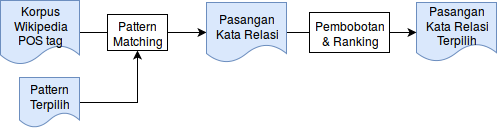
\includegraphics[scale=0.6]{pics/Pic04-PatternMatching}
    \caption{Proses Pembentukan \textit{Pair}}
    \label{fig:pattern-matching}
\end{figure}

Sebuah \textit{node} merepresentasikan satu kata dalam kalimat. Untuk setiap kalimat, dibentuk sebuah suffix tree yang merepresentasikan kalimat tersebut dan selanjutnya dicocokan dengan \textit{pattern} yang ada. Dibuat pula kelas \textit{Pair} yang merepresentasikan pasangan kata relasi \textit{hypernym-hyponym} yang dihasilkan dari proses \textit{pattern matching}. \textit{Pair} menyimpan informasi seperti total kemunculan, total dokumen unik, daftar kalimat unik dan \textit{pattern} unik yang menghasilkan \textit{pair}.

Tahapan proses \textit{pattern matching} jika diberikan satu kalimat dan satu \textit{pattern} adalah sebagai berikut.
\begin{enumerate}
  \item Kalimat masukan dibentuk menjadi suatu \textit{suffix tree}.
  \item \textit{Pattern} masukan ditokenisasi ke dalam bentuk \textit{list} kata. \textit{Pattern} pasti mengandung token <hypernym> dan <hyponym>, selanjutnya disebut token relasi.
  \item Jika ditemukan token relasi pada \textit{list pattern} yang sedang dievaluasi, maka \textit{node} yang dikunjungi disimpan sementara sesuai dengan relasinya.
  \item Jika token bukan token relasi, maka di evaluasi apakah token sama dengan \textit{node} yang dikunjungi. Jika sama maka proses evaluasi dilanjutkan, namun jika berbeda maka \textit{pattern} tidak cocok.
  \item Jika seluruh token \textit{pattern} telah dievaluasi dan tidak mengalami kegagalan, makan dianggap berhasil dan kata yang terekstrak disimpan dalam bentuk \textit{pair}.
\end{enumerate}

Pada masa awal pengembangan, setelah dijalankan proses \textit{pattern matching} terhadap korpus Wikipedia dengan \textit{pattern} hasil ekstraksi, masalah pertama yang ditemukan adalah banyaknya \textit{pair} yang salah satu atau kedua kata relasinya tidak teramasuk dalam kelas kata benda. Beberapa \textit{pair} yang salah diantaranya $(Menoitios;salah)$ dimana 'salah' adalah \textit{adjective} dan $(saya,gitaris)$ dimana 'saya' adalah preposi. Untuk itu diputuskan menggunakan korpus Wikipedia yang sudah melalui tahap POS Tagging.

Masalah lain yang muncul adalah jika kata yang ingin diekstrak merupakan \textit{multi word}. \textit{Pair} kurang baik yang dihasilkan sebelum mengatasi masalah ini diantaranya $(bola;olahraga)$ yang seharusnya $(sepak\,\,bola;olahraga)$, $(Serikat;negara)$ yang seharusnya $(Amerika\,\,Serikat;negara)$, dan $(Monterrey,ibu)$ yang seharusnya $(Monterrey;ibu\,\,kota)$. Solusi yang digunakan untuk mengatasi masalah ini adalah dengan mengasumsikan kata-kata berurutan yang memiliki kelas kata sama dalam suatu kalimat merupakan \textit{multi word}. \textit{Multi word} disimpan dalam satu \textit{node} pada pembentukan \textit{suffix tree}.
% --- kode pattern matching --- %
\begin{lstlisting}[caption={Algoritme ekstraksi \textit{pair}}, language=bash]
main:
  patterns = loadAllPatterns()
  openFiles()
  for sentence in sentences:
    matchAllPattern(sentence, patterns)

matchAllPattern(sentence, patterns):
  suffix_tree = buildTree(sentence)
  foreach pattern in patterns:
    matchTree(suffix_tree, pattern)
  
buildTree(sentence):
  tokens = buildSequence(sentence)
  suffix_tree;
  for(i = 0..tokens.size()):
    addSequence(suffix_tree, tokens, i)
  return suffix_tree;
addSequence(suffix_tree, tokens, i):
  node = suffix_tree.root
  for (j=i..tokens.size()):
    if (!node.childs.contains(tokens[j])):
      node = node.childs.add(tokens[j])
    node = node.childs.get(tokens[j])

matchTree(stree, pattern):
  foreach child in stree.root.childs:
    recursiveMatch(pattern, 0, child, ``'', ``'')
recursiveMatch(pattern, i, node, hype, hypo):
  if (i >= pattern.size() && hype && hypo):
    pair = createPair(hype, hypo)
    savePair(pair)
  else:
    cek = pattern[i]
    if (cek == ``hypenrym'' && cek.tag == (NN|NNP)):
      hype = cek
    else if (cek == ``hyponym'' && cek.tag == (NN|NNP)):
      hypo = cek
    else 
      if (cek != node.name) return
    foreach c in node.childs:
      recursiveMatch(pattern, i+1, c, hype, hypo)
\end{lstlisting}
% -------------------------------------------------- %


%-----------------------------------------------------------------------------%
\subsection{Vektor Pair}
%-----------------------------------------------------------------------------%
Suatu \textit{pair} dapat direpresentasikan ke dalam bentuk vektor berdasarkan nilai-nilai yang dimilikinya. Nilai-nilai fitur yang dimiliki oleh sebuah \textit{pair} adalah total kemunculan \textit{pair}, total dokumen yang membentuk \textit{pair}, jumlah \textit{pattern} unik, dan jumlah kalimat unik. Untuk memperkaya fitur \textit{pair}, dilakukan pula Word Embedding. Nilai \textit{similarity} antar dua kata relasi ditambahkan sebagai sebagai salah satu fitur.

%-----------------------------------------------------------------------------%
\subsection{Filterisasi dan Validasi Pair}
%-----------------------------------------------------------------------------%
\textit{Pair} baru yang dihasilkan untuk proses ini berjumlah sangat banyak, namun tidak semua \textit{pair} yang dihasilkan memenuhi relasi \textit{hypernym-hyponym}. Beberapa \textit{pair} kebetulan terekstrak akibat memenuhi \textit{pattern} lekscal yang sama dengan salah satu \textit{pattern} yang digunakan untuk proses \textit{pattern matching}. Untuk mengeliminasi data yang tidak diyakini benar, dilakukan validasi sederhana untuk setiap \textit{pair} yang dihasilkan. \textit{Pair} dinyatakan benar jika terdapat lebih dari satu \textit{pattern} yang mengekstrak \textit{pair} tersebut.

Setelah mengeliminasi \textit{pair} yang hanya terbentuk dari satu \textit{pattern}, dilakukan pembobotan. Tidak semua \textit{pair} yang dihasilkan masuk ke dalam korpus kata relasi. Bobot satu \textit{pair} dihitung menggunakan rumus berikut. 
\[ Bobot = (\frac{jumlah\,\,pattern\,\,pembentuk\,\,pair}{jumlah\,\,pattern\,\,digunakan} + similarity\,\,score)/2 \]
\noindent Jika nilai bobot melebihi threshold, maka \textit{pair} dimasukan ke dalam korpus pasangan kata relasi.

%-----------------------------------------------------------------------------%
%\subsection{Pengurutan Pair}
%-----------------------------------------------------------------------------%
%Pada saat ditampilkan, \textit{pair} diurutkan untuk mengetahui \textit{pair} mana yang diyakini paling benar. Proses pengurutan dilakukan berdasarkan beberapa tahap, yaitu:
% Semakin besar jumlah \textit{pattern} unik yang menghasilkan \textit{pair}.
% Semakin besar jumlah kalimat untuk yang menghasilkan \textit{pair}.


%-----------------------------------------------------------------------------%
\subsection{Pemodelan Word Embedding}
%-----------------------------------------------------------------------------%
Untuk menambah fitur pada vektor \textit{pair} yang dapat menunjang proses evaluasi, dilakukan Word Embedding. Implementasinya menggunakan model Word2Vec berbasis Python. Proses ini dibuat secara otomatis dengan hanya mengmasukan dokumen Bahasa Indonesia berukuran besar. Dalam penelitian ini, dokumen Bahasa Indoensia yang digunakan adalah korpus Wikipedia yang telah di proses.

Model dibuat menggunakan korpus Wikipedia yang telah melalui proses POS Tagging. Korpus tersebut diolah sedemikian sehingga kata-kata yang dianggap \textit{multi word}, memiliki kelas kata sama berurutan, digabung dengan simbol garis bawah ('\_'). Hal ini dilatarbelakangi atas hasil \textit{pair} yang banyak merupakan \textit{multi word}. Jika hal ini tidak dilakukan, maka akan banyak kata yang tidak ditemukan dalam \textit{dictionary} yang dihasilkan \textit{model word embedding}.

Model yang terbentuk, digunakan untuk memberi nilai \textit{similarity} antara kata \textit{hypernym-hyponym} dalam satu \textit{pair}. Hal ini diharapkan dapat memberi informasi lebih mengenai kualitas \textit{pair} yang dihasilkan.
